\documentclass{article}
\usepackage{geometry}
\usepackage{paralist}
\usepackage[T1]{fontenc}
\usepackage{reledmac}
\usepackage{changepage}
\usepackage{layout}

\usepackage{multirow}

\usepackage{pgfplots}
\usepackage{tikz}
\usetikzlibrary{positioning}
\usetikzlibrary{shapes.geometric, arrows}
\usetikzlibrary{calc, shapes, backgrounds}
\tikzstyle{arrow} = [thick,->,>=stealth]

\usepackage{graphicx} 
\graphicspath{ {./images/} }

\usepackage{fancyhdr}
\fancyhead[L]{
	\begin{tabular}{l}
		\Large \textbf{\textsc{Advanced Networking and Future Internet}} \\
		\large Theoretical Exercise 10
	\end{tabular}
}
\fancyhead[R]{
	\begin{tabular}{r}
		16-124-836 \\
		Marcel \textsc{Zauder}
	\end{tabular}
}
\renewcommand{\headrulewidth}{0.4pt}
\fancyfoot[C]{\thepage}
\renewcommand{\footrulewidth}{0.4pt}
\setlength{\headsep}{35pt}
\setlength{\textheight}{600pt}

\usepackage{hyperref}

\begin{document}
	\pagestyle{fancy}
	
	\section*{10.1 Why are Special Encoding and the use of Zig-Zag Order necessary for the compression? Would the compression be possible using only DCT and Quantization?}
	\begin{adjustwidth}{2em}{2em}
	\end{adjustwidth}
	
	\section*{10.2 Different Encoding Algorithms}
	\begin{adjustwidth}{2em}{2em}
		\subsection*{10.2.1 Huffman Encoding Representation}
		\begin{adjustwidth}{2em}{2em}
			\begin{tabular}{ccc}
				\begin{tabular}{|r|r|}
					\hline
					\textbf{Symbol} & \textbf{Frequency} \\
					\hline
					E & 22 \\
					N & 14 \\
					A & 13 \\
					D & 12 \\
					V & 10 \\
					C & 9 \\
					T & 8 \\
					K & 7 \\
					I & 6 \\
					G & 5 \\
					'space' & 4 \\
					W & 3 \\
					O & 2 \\
					R & 1 \\
					\hline		
				\end{tabular}
				&
				&
				\begin{tabular}{|r|r|}
					\hline
					\textbf{Symbol} & \textbf{Encoding} \\
					\hline		
					V & 111 \\
					D & 110 \\
					A & 101 \\
					N & 010 \\
					E & 001 \\
					I & 1001 \\
					K & 0111 \\
					T & 0110 \\
					C & 0001 \\
					W & 10001 \\
					'space' & 00001 \\
					G & 00000 \\
					R & 000001 \\
					O & 000000 \\		
					\hline
				\end{tabular}
			\end{tabular}
			\hfill \\
			\textbf{Tree:} \\
			\begin{tikzpicture}[
    			scale = 1, transform shape, thick, every node/.style = {draw, circle, minimum size = 5mm},
    			grow = down,  % alignment of characters
    			level 1/.style = {sibling distance=6cm},
    			level 2/.style = {sibling distance=2cm}, 
    			level 3/.style = {sibling distance=1cm},
    			level 4/.style = {sibling distance=1cm}, 
    			level 5/.style = {sibling distance=1cm},
    			level 6/.style = {sibling distance=1cm},
    			level distance = 1.25cm
  			]
  				\node[fill = gray!40, shape = circle, minimum width = 1cm, font = \sffamily] (116) {116}
  				child { node[shape = circle, draw, line width=1pt, minimum size=8mm, inner sep=0mm] (69) {69}
  					child { node [] (40) {40}
  						child { node [] (18) {18}
  							child { node [] (9) {9}
  								child { node [] (G) {G} }
  								child { node [] (_) {\_} }
  							}
  							child { node [] (C) {C} }
  						}
  						child { node [] (E) {E} }
  					}
  					child { node [] (29) {29}
  						child { node [] (N) {N}	}
  						child { node [] (15) {15}
  							child { node [] (T) {T} }
  							child { node [] (K) {K} }
  						}
  					}
  				}
  				child {node[shape = circle, draw, line width=1pt, minimum size=10mm, inner sep=0mm] (47) {47}
  					child { node [] (25) {25}
  						child { node [] (12) {12}
  							child { node [] (6) {6}
  								child { node [] (3) {3}
  									child { node [] (O) {O} }
  									child { node [] (R) {R} }
  								}
  								child { node [] (W) {W} }
  							}
  							child { node [] (I) {I} }
  						}
  						child { node [] (A) {A} }
  					}
  					child { node [] (22) {22}
  						child { node [] (D) {D} }
  						child { node [] (V) {V} }
  					}
  				};

  				% Labels
  				\begin{scope}[nodes = {draw = none}]
    				\path (116)-- (69) node [near start, left]  {$0$};
    				\path (116)-- (47) node [near start, right]  {$1$};
    				\path (69) -- (40) node [near start, left]  {$0$};
    				\path (69) -- (29) node [near start, right]  {$1$};
    				\path (47) -- (25) node [near start, left]  {$0$};
    				\path (47) -- (22) node [near start, right]  {$1$};
    				\path (40) -- (18) node [near start, left]  {$0$};
    				\path (40) -- (E) node [near start, right]  {$1$};
    				\path (29) -- (N) node [near start, left]  {$0$};
    				\path (29) -- (15) node [near start, right]  {$1$};
    				\path (25) -- (12) node [near start, left]  {$0$};
    				\path (25) -- (A) node [near start, right]  {$1$};
    				\path (22) -- (D) node [near start, left]  {$0$};
    				\path (22) -- (V) node [near start, right]  {$1$};
    				\path (18) -- (9) node [near start, left]  {$0$};
    				\path (18) -- (C) node [near start, right]  {$1$};
    				\path (15) -- (T) node [near start, left]  {$0$};
    				\path (15) -- (K) node [near start, right]  {$1$};
    				\path (12) -- (6) node [near start, left]  {$0$};
    				\path (12) -- (I) node [near start, right]  {$1$};
    				\path (9)  -- (G) node [near start, left]  {$0$};
    				\path (9)  -- (_) node [near start, right]  {$1$};
    				\path (6)  -- (3) node [near start, left]  {$0$};
    				\path (6)  -- (W) node [near start, right]  {$1$};
    				\path (3)  -- (O) node [near start, left]  {$0$};
    				\path (3)  -- (R) node [near start, right]  {$1$};
  				\end{scope}
			\end{tikzpicture}
		\end{adjustwidth}
		\subsection*{10.2.2 Arithmetic Encoding Representation}
		\begin{adjustwidth}{-2em}{}
			\begin{tabular}{|l|r|r|l|r|}
				\hline
				\multirow{2}{*}{\textbf{Symbol}} & \multirow{2}{*}{\textbf{Frequency}} & \textbf{Probability} & \multicolumn{2}{|c|}{\textbf{Interval reduced to ten-bit precision}} \\
				\cline{3-5}
				& & \textbf{(as fraction)} & \textbf{(as fractions)} & \textbf{(in binary)} \\
				\hline
				E & 22 & 22/116 & $[0, 194/1024)$ & $[0.0000000000, 0.0011000010)$ \\
				N & 14 & 14/116 & $[194/1024, 318/1024)$ & $[0.0011000010, 0.0100111101)$ \\
				A & 13 & 13/116 & $[318/1024, 433/1024)$ & $[0.0100111101, 0.0110110000)$ \\
				D & 12 & 12/116 & $[433/1024, 538/1024)$ & $[0.0110110000, 0.1000011010)$ \\
				V & 10 & 10/116 & $[538/1024, 627/1024)$ & $[0.1000011010, 0.1001110011)$ \\
				C & 9 & 9/116 & $[627/1024, 706/1024)$ & $[0.1001110011, 0.1011000010)$ \\
				T & 8 & 8/116 & $[706/1024, 777/1024)$ & $[0.1011000010, 0.1100001001)$ \\
				K & 7 & 7/116 & $[777/1024, 839/1024)$ & $[0.1100001001, 0.1101000111)$ \\
				I & 6 & 6/116 & $[839/1024, 892/1024)$ & $[0.1101000111, 0.1101111100)$ \\
				G & 5 & 5/116 & $[892/1024, 936/1024)$ & $[0.1101111100, 0.1110101000)$ \\
				'space' & 4 & 4/116 & $[936/1024, 971/1024)$ & $[0.1110101000, 0.1111001011)$ \\
				W & 3 & 3/116 & $[971/1024, 998/1024)$ & $[0.1111001011, 0.1111100110)$ \\
				O & 2 & 2/116 & $[998/1024, 1015/1024)$ & $[0.1111100110, 0.1111110111)$ \\
				R & 1 & 1/116 & $[1015/1024, 1)$ & $[0.1111110111, 1.0000000000)$ \\
				\hline
			\end{tabular}
		\end{adjustwidth}
		\subsection*{10.2.3 How many bit are necessary to encode the string \\ "ADVANCED NETWORKING" under each encoding?}
		\begin{adjustwidth}{2em}{2em}
			In the arithmetic encoding only 10 bits are needed to encode the whole string, because this is the precision given for our arithmetic encoding. When using the Huffman-Encoding Algorithm in total "ADVANCED NETWORKING" is encoded to "101 110 111 110 010 0001 001 110 00001 010 001 0110 10001 100000 100001 0111 1001 010 00000" which has 73 bits.
		\end{adjustwidth}
	\end{adjustwidth}
	
	\section*{10.3 Traditional Video Encoding}
	\begin{adjustwidth}{2em}{2em}
		\subsection*{10.2.1 What are the roles of each type of frame in traditional video encoding (I, P, and B), and what kind of information is encoded in each of the types?}
		\begin{adjustwidth}{2em}{2em}
		\end{adjustwidth}
		\subsection*{10.2.1 Different frame losses have different effects in overall video res-construction, what is the effect of loss of frames I, P, and B?}
		\begin{adjustwidth}{2em}{2em}
		\end{adjustwidth}
	\end{adjustwidth}
	
	\section*{10.4 How can motion estimation be achieved with the use of Macro-Blocks (block-matching algorithm)?}
	\begin{adjustwidth}{2em}{2em}
	\end{adjustwidth}
	
	\section*{10.5 Explain the components and steps in MPEG-1 encoding and decoding.}
	\begin{adjustwidth}{2em}{2em}
	\end{adjustwidth}
	
	\section*{10.6 Bonus Question}
	\begin{adjustwidth}{2em}{2em}
	\end{adjustwidth}
\end{document}